\documentclass[10pt]{article}
\usepackage[a3paper, landscape, margin=1.5cm, top=2.0cm, bottom=1.5cm]{geometry}
\usepackage{tikz}
\usetikzlibrary{arrows.meta, fit, backgrounds, calc, positioning, matrix}
\usepackage[T1]{fontenc}
\usepackage{xcolor}
\usepackage{fancyhdr}
\usepackage{caption}
\usepackage{float}


\definecolor{NavyD}     {HTML}{0D1B2A}
\definecolor{MGRAY}     {HTML}{999999}
\definecolor{SigGray}   {HTML}{5F5E5A}
\definecolor{CliD}      {HTML}{0F6E56}
\definecolor{CliF}      {HTML}{E1F5EE}
\definecolor{PurD}      {HTML}{5B2080}
\definecolor{PurF}      {HTML}{EEE0FA}
\definecolor{BluD}      {HTML}{185FA5}
\definecolor{BluF}      {HTML}{E6F1FB}
\definecolor{DramD}     {HTML}{B86A00}
\definecolor{DramF}     {HTML}{FDF0DC}
\definecolor{SlotAmberF}{HTML}{FAEEDA}
\definecolor{SlotAmberD}{HTML}{BA7517}
\definecolor{SlotGreenF}{HTML}{EAF3DE}
\definecolor{SlotGreenD}{HTML}{3B6D11}
\definecolor{SlotGrayF} {HTML}{F1EFE8}
\definecolor{SlotGrayD} {HTML}{888780}
\definecolor{AnnD}      {HTML}{185FA5}
\definecolor{AnnF}      {HTML}{E6F1FB}

\tikzset{
  BLKS/.style args={#1/#2}{
    rectangle, rounded corners=5pt,
    draw=#1, fill=#2, text=#1,
    font=\small\bfseries, align=center,
    inner sep=6pt, minimum width=3.0cm, minimum height=1.5cm,
    line width=0.65pt
  },
  EXTBLK/.style args={#1/#2}{
    rectangle, rounded corners=5pt,
    draw=#1, fill=#2, text=#1,
    font=\small\bfseries, align=center,
    inner sep=6pt, minimum width=2.8cm, minimum height=1.1cm,
    line width=0.65pt, dashed
  },
  SLOT/.style args={#1/#2}{
    rectangle, draw=#2, fill=#1,
    minimum width=2.6cm, minimum height=0.58cm,
    font=\fontsize{6.5}{8}\selectfont,
    align=center, inner sep=2pt, line width=0.45pt
  },
  ARR/.style={-{Stealth[length=5pt,width=4pt]}, line width=0.85pt, color=#1},
  ARRD/.style={-{Stealth[length=4pt,width=3.5pt]}, line width=0.6pt, color=#1, dashed},
  BUS/.style={line width=0.85pt, color=#1},
  lbl/.style={font=\fontsize{6.5}{8}\selectfont\itshape,
              text=SigGray, fill=white, inner sep=1.5pt},
  ANN/.style={draw=AnnD, fill=AnnF, rounded corners=4pt,
              font=\fontsize{7}{9}\selectfont,
              text=NavyD, inner sep=8pt, align=left, line width=0.6pt},
  HDARR/.style={-{Stealth[length=4pt,width=3.5pt]}, line width=0.8pt, color=SlotAmberD},
}

\pagestyle{fancy}\fancyhf{}
\renewcommand{\headrulewidth}{0.3pt}
\fancyhead[L]{\scriptsize\color{MGRAY}Reconfigurable DDR Memory Controller}
\fancyhead[R]{\scriptsize\color{MGRAY}Microarchitecture Specification}
\fancyfoot[C]{\scriptsize\thepage}
\captionsetup{font=scriptsize, labelfont=bf, skip=5pt}

\begin{document}
\thispagestyle{fancy}

\begin{center}
  {\large\bfseries\color{NavyD}
    Reorder Buffer (ROB) \textemdash\ Internal Architecture}\\[3pt]
  {\small\color{MGRAY} Client Interface (CIF) \textemdash\ Read Return Path}
\end{center}
\vspace{2pt}

%% ═══════════════════════════════════════════════════════
%% LAYOUT STRATEGY: Relative Positioning (not absolute)
%% ═══════════════════════════════════════════════════════
%% Key elements:
%%   - Issue path blocks (rcp, seqgen, taginst) positioned left-to-right
%%   - Queue matrix: 3 columns (Q0, Q1, QN) × 4 rows (slots)
%%   - Fill block: below queues (relative to matrix)
%%   - Retirement Logic: right of queue matrix
%%   - Buses and connections: positioned relative to nodes
%%   - ROB boundary: fit node around all internal elements
%%   - Annotation: positioned right of ROB boundary
%% Benefits:
%%   - No hardcoded coordinates
%%   - Easy to adjust spacing (change node sep, distances)
%%   - Maintainable and scalable for future diagrams
%% ═══════════════════════════════════════════════════════

\begin{figure}[H]
\centering
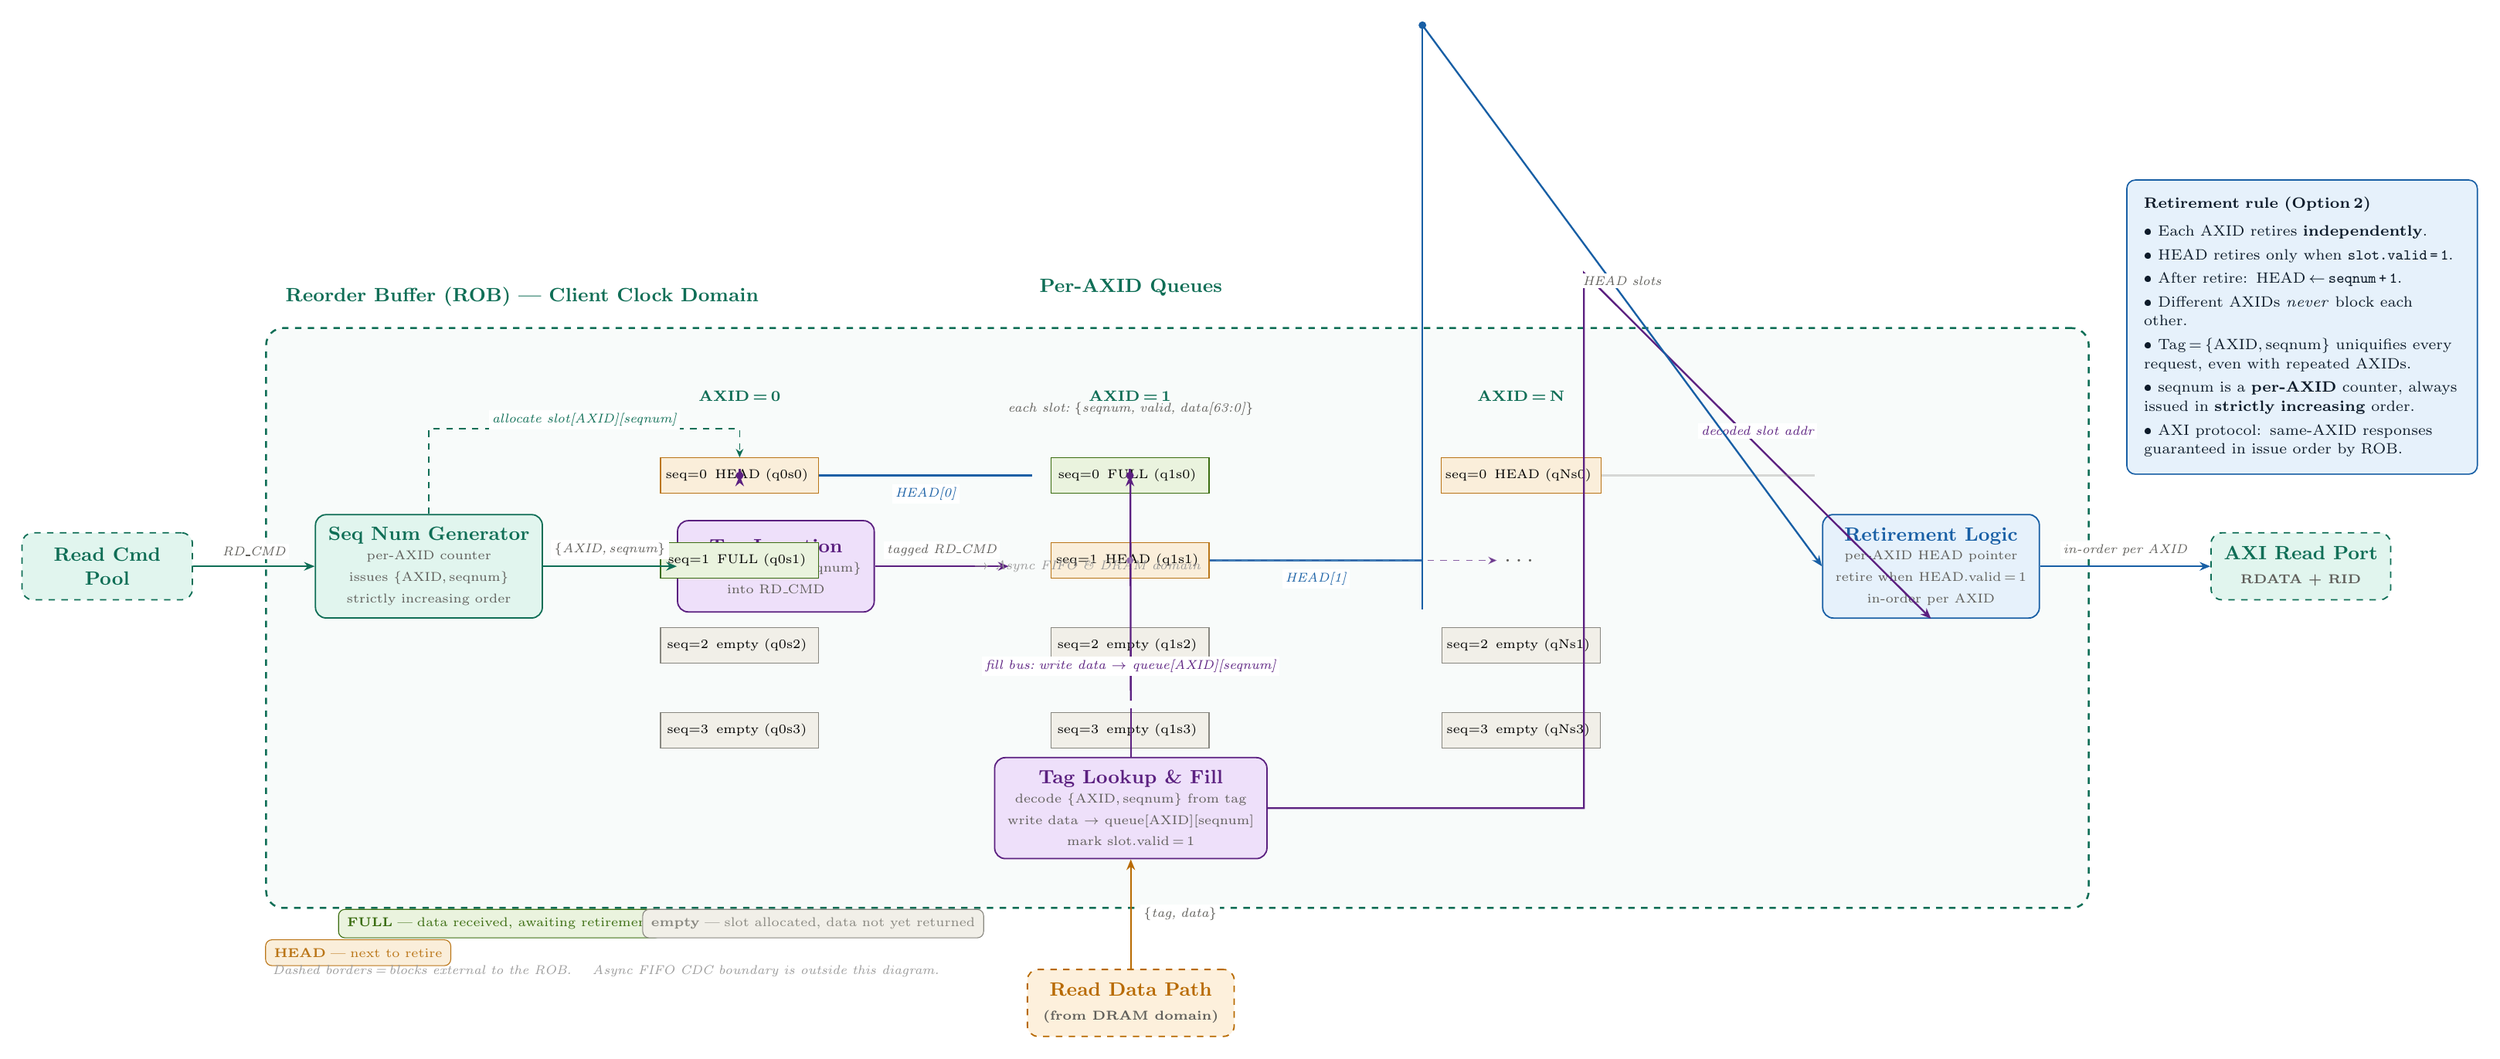
\begin{tikzpicture}[x=1cm, y=1cm]

%% ═══════════════════════════════════════════════════════
%% REFACTORED LAYOUT: Using positioning and matrix
%% ═══════════════════════════════════════════════════════

%% ── ISSUE PATH (left side) ─────────────────────────────
\node[EXTBLK=CliD/CliF] (rcp)
  {Read Cmd\\Pool};

\node[BLKS=CliD/CliF, right=2cm of rcp] (seqgen) {%
  Seq Num Generator\\[-2pt]
  {\fontsize{6.5}{8}\selectfont\mdseries\color{SigGray}per-AXID counter}\\[-1pt]
  {\fontsize{6.5}{8}\selectfont\mdseries\color{SigGray}issues \{AXID,\,seqnum\}}\\[-1pt]
  {\fontsize{6.5}{8}\selectfont\mdseries\color{SigGray}strictly increasing order}%
};

\node[BLKS=PurD/PurF, right=2.2cm of seqgen] (taginst) {%
  Tag Insertion\\[-2pt]
  {\fontsize{6.5}{8}\selectfont\mdseries\color{SigGray}embeds \{AXID,\,seqnum\}}\\[-1pt]
  {\fontsize{6.5}{8}\selectfont\mdseries\color{SigGray}into RD\_CMD}%
};

%% ── QUEUE MATRIX (center) ──────────────────────────────
%% Queue structure: 3 columns (Q0, Q1, QN) × 4 rows (slots)
\matrix[
  matrix of nodes,
  nodes={anchor=center},
  column sep=3.8cm,
  row sep=0.8cm,
  below=4.5cm of seqgen,
  right=1.8cm of seqgen,
  name=queue-matrix
] {
  |[font=\fontsize{7.5}{9}\selectfont\bfseries, text=CliD]| AXID\,=\,0
    & |[font=\fontsize{7.5}{9}\selectfont\bfseries, text=CliD]| AXID\,=\,1
    & |[font=\fontsize{7.5}{9}\selectfont\bfseries, text=CliD]| AXID\,=\,N \\
  |[SLOT=SlotAmberF/SlotAmberD]| seq=0\enspace HEAD (q0s0)
    & |[SLOT=SlotGreenF/SlotGreenD]| seq=0\enspace FULL (q1s0)
    & |[SLOT=SlotAmberF/SlotAmberD]| seq=0\enspace HEAD (qNs0) \\
  |[SLOT=SlotGreenF/SlotGreenD]| seq=1\enspace FULL (q0s1)
    & |[SLOT=SlotAmberF/SlotAmberD]| seq=1\enspace HEAD (q1s1)
    & |[font=\large, text=SigGray]| \ldots \\
  |[SLOT=SlotGrayF/SlotGrayD]| seq=2\enspace empty (q0s2)
    & |[SLOT=SlotGrayF/SlotGrayD]| seq=2\enspace empty (q1s2)
    & |[SLOT=SlotGrayF/SlotGrayD]| seq=2\enspace empty (qNs1) \\
  |[SLOT=SlotGrayF/SlotGrayD]| seq=3\enspace empty (q0s3)
    & |[SLOT=SlotGrayF/SlotGrayD]| seq=3\enspace empty (q1s3)
    & |[SLOT=SlotGrayF/SlotGrayD]| seq=3\enspace empty (qNs3) \\
};

%% Queue header (above matrix)
\node[font=\small\bfseries, text=CliD, above=1.2cm of queue-matrix]
  {Per-AXID Queues};
\node[font=\fontsize{6.5}{8}\selectfont\itshape, text=SigGray, below=0.3cm of queue-matrix.north]
  {each slot:\;\{seqnum,\;valid,\;data[63:0]\}};

%% ── RETURN PATH AND FILL BLOCK (below queues) ─────────
\node[EXTBLK=DramD/DramF, minimum width=3.4cm, below=3.5cm of queue-matrix]
  (dram)
  {Read Data Path\\
   {\fontsize{6}{7.5}\selectfont\color{SigGray}(from DRAM domain)}};

\node[BLKS=PurD/PurF, minimum width=3.2cm, above=1.8cm of dram]
  (fill)
  {Tag Lookup \&\ Fill\\[-2pt]
   {\fontsize{6.5}{8}\selectfont\mdseries\color{SigGray}decode \{AXID,\,seqnum\} from tag}\\[-1pt]
   {\fontsize{6.5}{8}\selectfont\mdseries\color{SigGray}write data $\to$ queue[AXID][seqnum]}\\[-1pt]
   {\fontsize{6.5}{8}\selectfont\mdseries\color{SigGray}mark slot.valid\,=\,1}};

%% ── RETIREMENT LOGIC (right of queue matrix) ──────────
\node[BLKS=BluD/BluF, minimum width=3.2cm, right=3.5cm of queue-matrix]
  (retire)
  {Retirement Logic\\[-2pt]
   {\fontsize{6.5}{8}\selectfont\mdseries\color{SigGray}per-AXID HEAD pointer}\\[-1pt]
   {\fontsize{6.5}{8}\selectfont\mdseries\color{SigGray}retire when HEAD.valid\,=\,1}\\[-1pt]
   {\fontsize{6.5}{8}\selectfont\mdseries\color{SigGray}in-order per AXID}};

%% ── EXTERNAL OUTPUT (far right) ────────────────────────
\node[EXTBLK=CliD/CliF, minimum width=2.8cm, right=2.8cm of retire]
  (axiout)
  {AXI Read Port\\
   {\fontsize{6}{7.5}\selectfont\color{SigGray}RDATA + RID}};

%% ── ISSUE PATH ARROWS ─────────────────────────────────
\draw[ARR=CliD] (rcp.east) -- (seqgen.west)
  node[lbl, midway, above=3pt] {RD\_CMD};

\draw[ARR=CliD] (seqgen.east) -- (taginst.west)
  node[lbl, midway, above=3pt] {\{AXID,\,seqnum\}};

\draw[ARR=PurD] (taginst.east) -- ++(2.2,0)
  node[lbl, midway, above=3pt] {tagged RD\_CMD};
\node[font=\fontsize{6}{7.5}\selectfont\itshape, text=MGRAY, right=1.5cm of taginst]
  {$\to$ Async FIFO \& DRAM domain};

%% ── ALLOCATE ARROW (to queue column 0) ────────────────
\draw[ARRD=CliD]
  (seqgen.north) -- ++(0, 1.4)
  -| (queue-matrix-2-1.north);
\node[lbl, text=CliD, anchor=south] at ($(seqgen)!0.5!(queue-matrix-2-1) + (0, 1.5)$)
  {allocate slot[AXID][seqnum]};

%% ── RETURN PATH: DRAM → FILL ──────────────────────────
\draw[ARR=DramD] (dram.north) -- (fill.south)
  node[lbl, midway, right=4pt] {\{tag,\;data\}};

%% ── RETURN PATH: FILL → RETIREMENT ────────────────────
\draw[ARR=PurD] (fill.east) -- ++(5.2, 0) -- ++(0, 8.8) -- (retire.south)
  node[lbl, pos=0.5, above=3pt, text=PurD] {decoded slot addr};

%% ── FILL BUS ──────────────────────────────────────────
%% Positioned relative to queue matrix and fill block
\draw[BUS=PurD]
  (fill.north) -- ($(fill.north) + (0, 0.8)$);
  
\node (fill-bus-h) at ($(fill.north) + (0, 0.8)$) {};
\draw[BUS=PurD]
  ($(queue-matrix-2-1)!0.5!(queue-matrix-2-3)$) 
  -- (fill-bus-h);

\node[lbl, text=PurD, above=0.4cm of fill-bus-h]
  {fill bus:\;write data $\to$ queue[AXID][seqnum]};

%% Junction dots - relative to queue matrix columns
\fill[PurD]   (queue-matrix-2-1) circle (1.8pt);
\fill[PurD]   (queue-matrix-2-2) circle (1.8pt);
\fill[PurD!65] (queue-matrix-3-2) circle (1.6pt);

%% Branches to queues
\draw[ARR=PurD] (queue-matrix-2-1) -- (queue-matrix-2-1);  % Q0, row 2 to row 1
\draw[ARR=PurD] (queue-matrix-2-2) -- (queue-matrix-2-2);  % Q1, row 2 to row 1
\draw[ARRD=PurD, opacity=0.7] (queue-matrix-3-2) -- (queue-matrix-3-3);  % QN

%% ── RETIREMENT BUS ────────────────────────────────────
%% HEAD slots extend right from queues
\draw[BUS=BluD]
  (queue-matrix-2-1.east) -- ($(queue-matrix-2-1.east) + (3.5, 0)$);
\node[lbl, text=BluD] at ($(queue-matrix-2-1.east) + (1.75, -0.3)$) 
  {HEAD[0]};

\draw[BUS=BluD, opacity=0.8]
  (queue-matrix-3-2.east) -- ($(queue-matrix-3-2.east) + (3.5, 0)$);
\node[lbl, text=BluD] at ($(queue-matrix-3-2.east) + (1.75, -0.3)$) 
  {HEAD[1]};

\draw[BUS=SlotGrayD, opacity=0.3]
  (queue-matrix-2-3.east) -- ($(queue-matrix-2-3.east) + (3.5, 0)$);

%% Vertical bus spine
\node (ret-bus-v) at ($(queue-matrix-3-2.east) + (3.5, 0)$) {};
\draw[BUS=BluD]
  ($(ret-bus-v) + (0, -0.8)$) -- ($(ret-bus-v) + (0, 8.8)$);
\fill[BluD] ($(ret-bus-v) + (0, 8.8)$) circle (1.8pt);

%% Into Retirement Logic
\draw[ARR=BluD]
  ($(ret-bus-v) + (0, 8.8)$) -- (retire.west)
  node[lbl, midway, above=3pt] {HEAD slots};

%% ── RETIREMENT → AXI OUTPUT ───────────────────────────
\draw[ARR=BluD] (retire.east) -- (axiout.west)
  node[lbl, pos=0.5, above=3pt] {in-order per AXID};

%% ── ROB BOUNDARY BOX (using fit) ──────────────────────
\begin{scope}[on background layer]
  \node[
    fit=(seqgen) (taginst) (queue-matrix) (fill) (retire),
    inner sep=0.8cm,
    rounded corners=8pt,
    draw=CliD,
    dashed,
    line width=0.9pt,
    fill=CliD!3
  ] (rob-boundary) {};
  
  \node[font=\small\bfseries, text=CliD, above right=0.3cm of rob-boundary.north west]
    {Reorder Buffer (ROB) \textemdash\ Client Clock Domain};
\end{scope}

%% ── ANNOTATION BOX ────────────────────────────────────
\node[ANN, text width=5.2cm, right=0.6cm of rob-boundary.north east]
  {%
    \textbf{Retirement rule (Option\,2)}\\[4pt]
    \textbullet\ Each AXID retires \textbf{independently}.\\[2pt]
    \textbullet\ HEAD retires only when \texttt{slot.valid\,=\,1}.\\[2pt]
    \textbullet\ After retire: HEAD\,$\leftarrow$\,\texttt{seqnum\,+\,1}.\\[2pt]
    \textbullet\ Different AXIDs \emph{never} block each other.\\[2pt]
    \textbullet\ Tag\,=\,\{AXID,\,seqnum\} uniquifies every
      request, even with repeated AXIDs.\\[2pt]
    \textbullet\ seqnum is a \textbf{per-AXID} counter,
      always issued in \textbf{strictly increasing} order.\\[2pt]
    \textbullet\ AXI protocol: same-AXID responses
      guaranteed in issue order by ROB.%
  };

%% ── SLOT LEGEND (below ROB) ────────────────────────────
\node[draw=SlotAmberD, fill=SlotAmberF, rounded corners=3pt,
      font=\fontsize{6.5}{8}\selectfont, text=SlotAmberD,
      inner sep=4pt, below=0.5cm of rob-boundary.south west, anchor=north west]
  {\textbf{HEAD}\;—\;next to retire};

\node[draw=SlotGreenD, fill=SlotGreenF, rounded corners=3pt,
      font=\fontsize{6.5}{8}\selectfont, text=SlotGreenD,
      inner sep=4pt, right=1.2cm of rob-boundary.south west, anchor=north west]
  {\textbf{FULL}\;—\;data received, awaiting retirement};

\node[draw=SlotGrayD, fill=SlotGrayF, rounded corners=3pt,
      font=\fontsize{6.5}{8}\selectfont, text=SlotGrayD,
      inner sep=4pt, right=6.2cm of rob-boundary.south west, anchor=north west]
  {\textbf{empty}\;—\;slot allocated, data not yet returned};

%% ── FOOTNOTE ──────────────────────────────────────────
\node[font=\fontsize{6}{7.5}\selectfont\itshape,
      text=MGRAY, below=0.8cm of rob-boundary.south west, anchor=north west]
  {Dashed borders\,=\,blocks external to the ROB.
   \quad Async FIFO CDC boundary is outside this diagram.};

\end{tikzpicture}

\caption{%
  Internal architecture of the Reorder Buffer (ROB), operating entirely
  within the client clock domain.
  \textbf{Issue path:} the \textbf{Seq Num Generator} assigns a per-AXID
  \texttt{seqnum} in strictly increasing order, allocates the corresponding
  \texttt{queue[AXID][seqnum]} slot, and passes \{AXID,\,seqnum\} to
  \textbf{Tag Insertion}, which embeds the composite tag into the outgoing
  \texttt{RD\_CMD} before it crosses the Async FIFO CDC boundary (outside ROB).
  \textbf{Return path:} read data arrives from the DRAM domain as
  \{tag,\,data\}; \textbf{Tag Lookup \&\ Fill} decodes the tag, writes data
  into \texttt{queue[AXID][seqnum]}, and sets \texttt{slot.valid\,=\,1}.
  \textbf{Retirement Logic} advances a per-AXID HEAD pointer whenever
  \texttt{HEAD.valid\,=\,1}, guaranteeing in-order delivery per AXID
  (Option\,2) while allowing independent AXIDs to retire without mutual blocking.}
\label{fig:rob}
\end{figure}
\end{document}